\documentclass[exercice]{thedocument}%
\begin{document}%
    \enonce{0089}%
    \begin{enumerate}[label=\arabic*),font=\bfseries]
        \item
        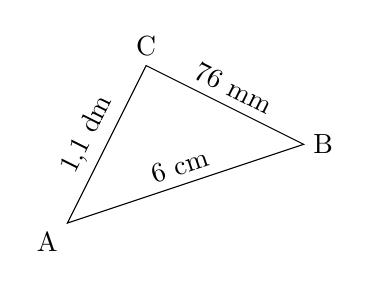
\begin{tikzpicture}[baseline=(C.base)]
            \coordinate[label=below left:A](A)at(0,0);
            \coordinate[label=right:B](B)at(3,1);
            \coordinate[label=above:C](C)at(1,2);
            \draw(A)--(B)--(C)--cycle;
            \path(A)--(B)node[pos=0.5,sloped,above]{6 cm};
            \path(B)--(C)node[pos=0.5,sloped,above]{76 mm};
            \path(A)--(C)node[pos=0.5,sloped,above]{1,1 dm};
        \end{tikzpicture}
        \item
        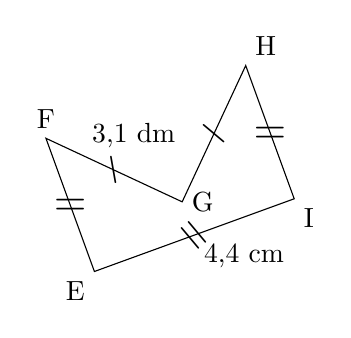
\begin{tikzpicture}[baseline=(F.base),rotate=20,scale=0.9]
            \coordinate[label=below left:E](E)at(-1.5,0);
            \coordinate[label=above:F](F)at(-1.5,2);
            \coordinate[label=right:G](G)at(0,0.5);
            \coordinate[label=above right:H](H)at(1.5,2);
            \coordinate[label=below right:I](I)at(1.5,0);
            \draw(E)--(F)--(G)--(H)--(I)--cycle;
            \path(E)--(F)node[pos=0.5,rotate=90]{{\boldmath$||$}};
            \path(H)--(I)node[pos=0.5,rotate=90]{{\boldmath$||$}};
            \path(E)--(I)node[pos=0.5,rotate=40]{{\boldmath$||$}}
                node[below right,pos=0.5]{4,4 cm};
            \path(F)--(G)node[pos=0.5,rotate=10]{{\boldmath$|$}}
                node[shift={(60:0.5)},pos=0.5]{3,1 dm};
            \path(G)--(H)node[pos=0.5,rotate=50]{{\boldmath$|$}};
        \end{tikzpicture}
    \end{enumerate}
\end{document}